\section{{\large \SeeDB\ } Design}
\label{sec:system_architecture}

In this section, we present the \SeeDB\ architecture, starting with an
overview followed by a detailed discussion of its components.

\subsection{{\large \SeeDB} architecture overview}
\label{subsec:overview}

Our \SeeDB\ prototype is designed as a layer on top of a traditional
relational database system.
While optimization opportunities are restricted by virtue of being outside the
database, our design permits \SeeDB\ to be used in conjunction with a variety of
existing database systems. 
\SeeDB\ is comprised of two parts: a frontend and a backend. 
The frontend is a ``thin client'' that
is used to issue queries and display visualizations. The backend, in
contrast, performs all the computation required to generate and select views
to be recommended. Figure \ref{fig:sys-arch}
depicts the architecture of our system.

\begin{figure}[htb]
\vspace{-10pt}
\centerline{
\hbox{\resizebox{9cm}{!}{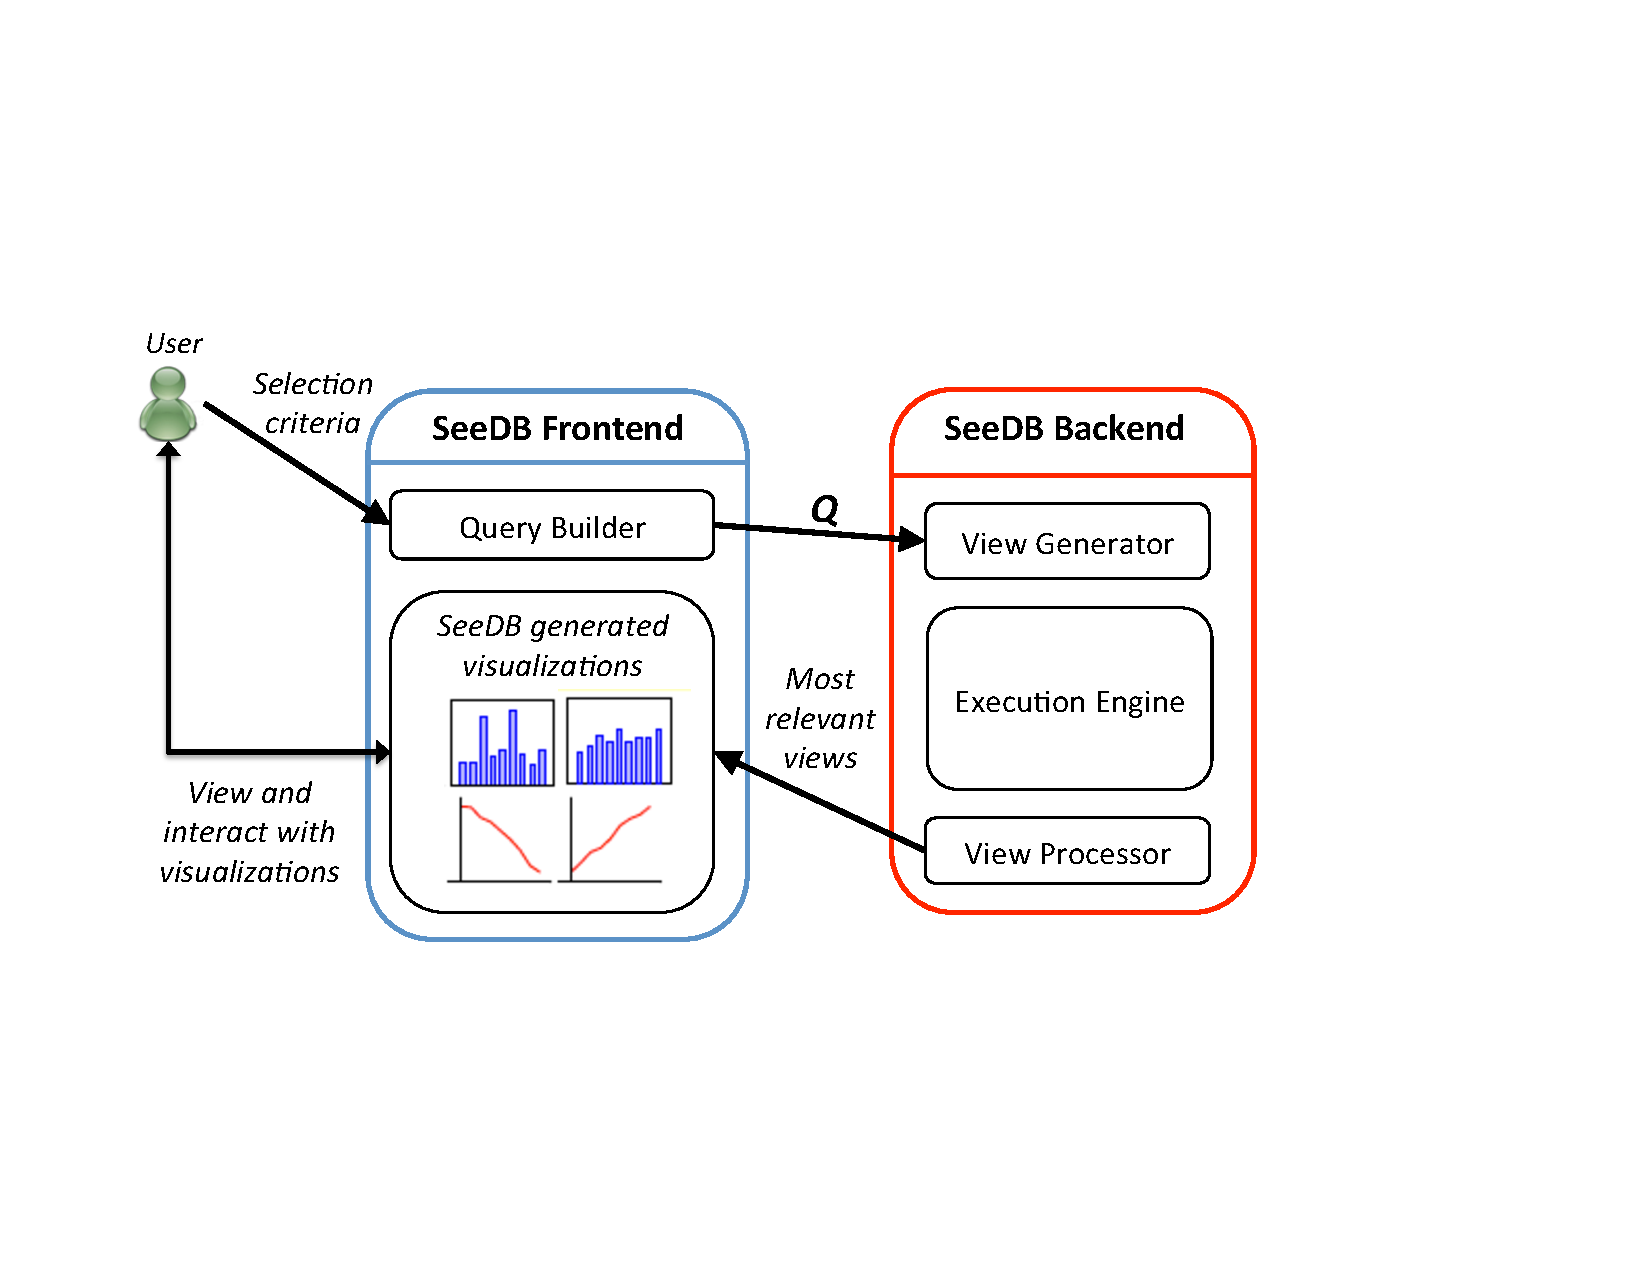
\includegraphics[trim=10mm 50mm 10mm 50mm,
clip=true]{Images/seedb-architecture.pdf}}}}
\caption{SeeDB Architecture}
\label{fig:sys-arch}
\vspace{-12pt}
\end{figure} 

An analyst uses the frontend to issue queries to \SeeDB. We provide three
mechanisms for the analyst to issue queries (further discussion in
Section \ref{subsec:seedb_frontend}).
Once the analyst issues a query via the frontend, the backend takes over.
First, the Metadata Collector module queries metadata tables (a combination of
database-provided and \SeeDB\ specific tables) for information such as table
sizes, column types, data distribution, and table access patterns.
The resulting metadata along with the analyst's query is then passed to the
Query Generator module. The purpose of the Query Generator is two-fold:
first, it uses metadata to prune the space of candidate views to only retain the
most promising ones; and second, it generates target and comparison views for
each view that has not been pruned.
The SQL queries corresponding to the target and comparison views are then passed
to the Optimizer module. We refer to these queries collectively as {\it view
queries}.
Next, the Optimizer module determines the best way to
combine view queries intelligently so that the total execution time is
minimized.
(We discuss optimizations performed by \SeeDB\ in Section
\ref{subsec:seedb_backend}.) Once the Optimizer module has generated the
optimized queries, \SeeDB\ runs them on the underlying DBMS.
Results of the optimized queries are processed by the View Processor in a
streaming fashion to produce results for individual views. Individual view
results are then normalized and the utility of each view is computed.
Finally \SeeDB\ selects the top $k$ views with the highest utility and returns
them to the \SeeDB\ frontend. The frontend generates 
and displays visualizations for each of these view. We now discuss
\SeeDB\ modules in detail.